%!TEX root = ../dokumentation.tex

\chapter{Erstellung der Anwendung}
In den vorherigen Kapiteln wurden grundlegende Ansätze der digitalen Bildverarbeitung und Schach-Engines erläutert.
Dieses Kapitel beschäftigt sich mit der Implementierung des gewonnenen Wissens, um das Ziel der Applikation zu erreichen.  
Es wird aufgezeigt, wie das Projekt über einen objektorientierten Ansatz und mithilfe von Pygame zur 
Erstellung des Spiels, sowie OpenCV zur Kameraauswertung, umgesetzt wurde.

\section{Design und Architektur}
Das Projekt verfolgt einen objektorientierten Ansatz. Es existieren sieben Hauptklassen und eine Klasse für Konstanten.
Im Folgenden werden die Klassen und deren Aufgabe in Bezug auf die Applikation aufgeführt.

\subsection{Figuren Klasse}
Die Figuren Klasse stellt eine Schachfigur dar. Dabei hat jede Figur eine \(COLOR\), die entweder schwarz oder weiß ist.
Die weiße Farbe wird dabei mit \(0b0\) dargestellt und die schwarze Farbe mit \(0b1\). Dieses Farbschema zieht sich über das komplette Projekt.
Neben der Farbe hat jede Figur einen Namen, der dem Namen der jeweiligen Bilddatei entspricht. Ein weißer Bauer hat also den Namen \(0\_pawn.png \).  
Der Parameter \(TYPE\) ist ein String, der den Figurentyp beschreibt.

\begin{itemize}
    \item {\(p\) beschreibt einen Bauern.}
    \item {\(r\) beschreibt einen Turm.}
    \item {\(n\) beschreibt einen Springer.}
    \item {\(b\) beschreibt einen Läufer.}
    \item {\(q\) beschreibt eine Dame.}
    \item {\(k\) beschreibt einen König.}
\end{itemize}

Außerdem besitzt jede Figur eine Liste \(moves\), die alle legalen Züge der Figur beinhaltet. Die Züge sind Objekte einer Hilfsklasse, auf die später 
genauer eingegangen wird. Der Boolean \(HAS\_RANGE\_MOVEMENT\) gibt an, ob die Figur ein Läufer, Turm oder eine Dame ist. Wenn das der Fall ist,
ist der Wert wahr, ansonsten ist er falsch. Das letzte Attribut \(has\_moved\) beschreibt, ob eine Figur bereits gezogen wurde.
\begin{figure}[ht]
    \centering
    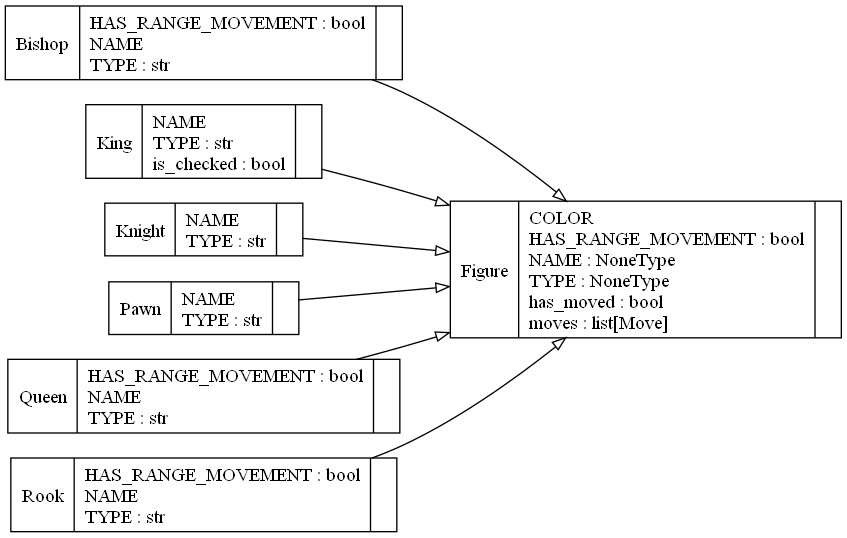
\includegraphics[scale=0.6]{images/classes_figures.png}
    \caption{Figuren Klassen}
\end{figure}
Neben der allgemeinen Figuren Klasse, gibt es für jede Figur noch eine einzelne Klasse, die jeweils von der Figuren Klasse erbt.
Um einen schwarzen Bauern zu erstellen, wird also ein Objekt mit dem Konstruktor der Bauern Klasse erstellt, die nur noch die Farbe als Parameter nimmt.
Die restlichen Attribute werden automatisch gesetzt. Der König hat dabei noch ein extra Attribut \(is\_checked\), das wahr wird, wenn er angegriffen wird.

\subsection{Schachbrett Klasse}
\begin{figure}[ht]
    \centering
    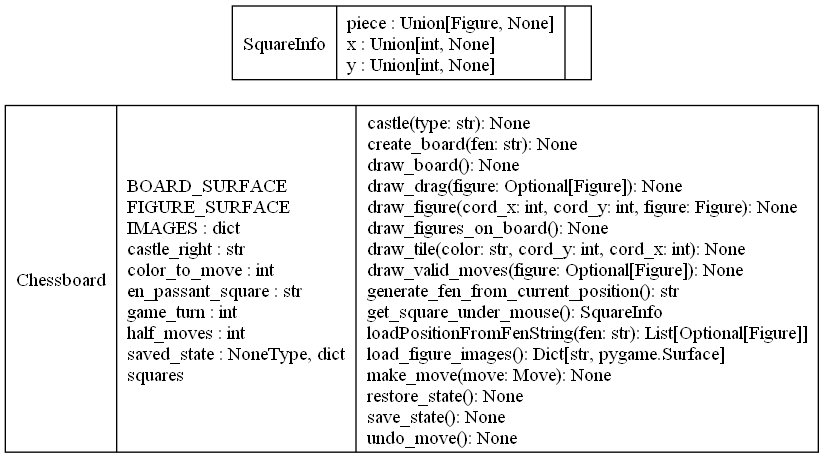
\includegraphics[scale=0.6]{images/classes_chessboard.png}
    \caption{Schachbrett Klasse}
\end{figure}
Die Klasse \(chessboard.py\) beinhaltet alle Attribute und Funktionen, die mit dem Schachbrett zu tun haben. Dazu gehört das Zeichnen des Schachbretts, 
das Zeichen der Figuren auf dem Schachbrett, das Speichern der aktuellen Position und das Spielen oder zurücknehmen von Zügen.

\subsection{Klasse zur Kameraimplementierung}
Die Klasse \(ChessCam.py\) dient dazu, mithilfe einer Kamera die Züge des Spielers zu erkennen. Es gibt eine Funktion, die das Schachbrett erkennt und 
Funktionen mit deren Hilfe die Unterschiede zu einer vorherigen Position ausgewertet werden, um dann den Spielzug zu erkennen.
\begin{figure}[ht]
    \centering
    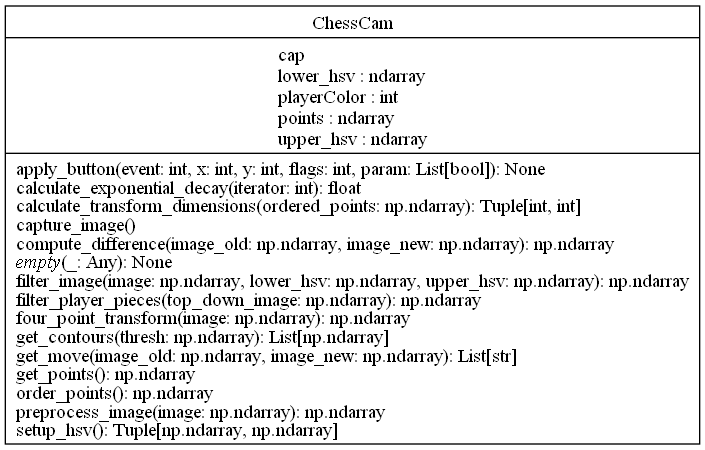
\includegraphics[scale=0.6]{images/class_cam.png}
    \caption{ChessCam Klasse}
\end{figure}

\subsection{Klasse zur Zuggenerierung}
\(moveGenerator.py\) dient dazu, die legalen Züge des aktuellen Spielers zu berechnen. Das ist notwendig, um dem Spieler die verfügbaren Züge anzuzeigen und 
illegale eventuell falsch erkannte Züge zu verbieten. Die legalen Züge werden anschließend der jeweiligen Figur als Attribut gegeben.
Sobald ein Spieler keinen legalen Zug mehr hat, ist das Spiel zu Ende und der andere Spieler gewinnt. Die generierten Züge sind dabei vom Datentyp \(Move\).

\subsection{Move Klasse}
\begin{figure}[H]
    \centering
    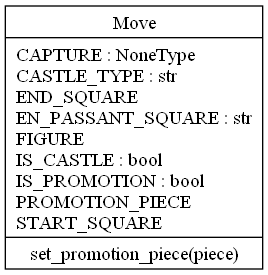
\includegraphics[scale=0.7]{images/class_move.png}
    \caption{Move Klasse}
\end{figure}

Diese Klasse dient als Hilfsklasse, um einen Zug zu beschreiben. Sie beinhaltet dabei das Startfeld, das Endfeld des Zuges, sowie die Figur, die den Zug ausführt.
Sollte es sich um einen Sonderzug handeln werden bestimmte flags gesetzt, die dies kennzeichnen. Ein Bauernzug, der zwei Felder nach vorne geht, beinhaltet
beispielsweise das \(EN\_PASSANT\_SQUARE\) flag.

\subsection{Computer Klasse}
Das Computer-Objekt wird genutzt, um die Züge der Engine zu berechnen. Dabei wird die Python Bibliothek von Stockfish genutzt, die die aktuelle Position 
als Input bekommt und dann anschließend einen Zug an die PyChess Klasse zurückgibt und dann auf dem Brett gespielt wird.

\subsection{PyChess Klasse}
Die Klasse \(pychess.py\) ist das Kernstück der Anwendung. In ihr wird das Spiel gestartet, das Schachbrett aus einer bestimmten Position gestartet,
und sie ist dafür verantwortlich, dass der Spieler mit der GUI interagieren kann, um seine Züge zu spielen.

\section{Spielverlauf}
\begin{figure}[H]
    \centering
    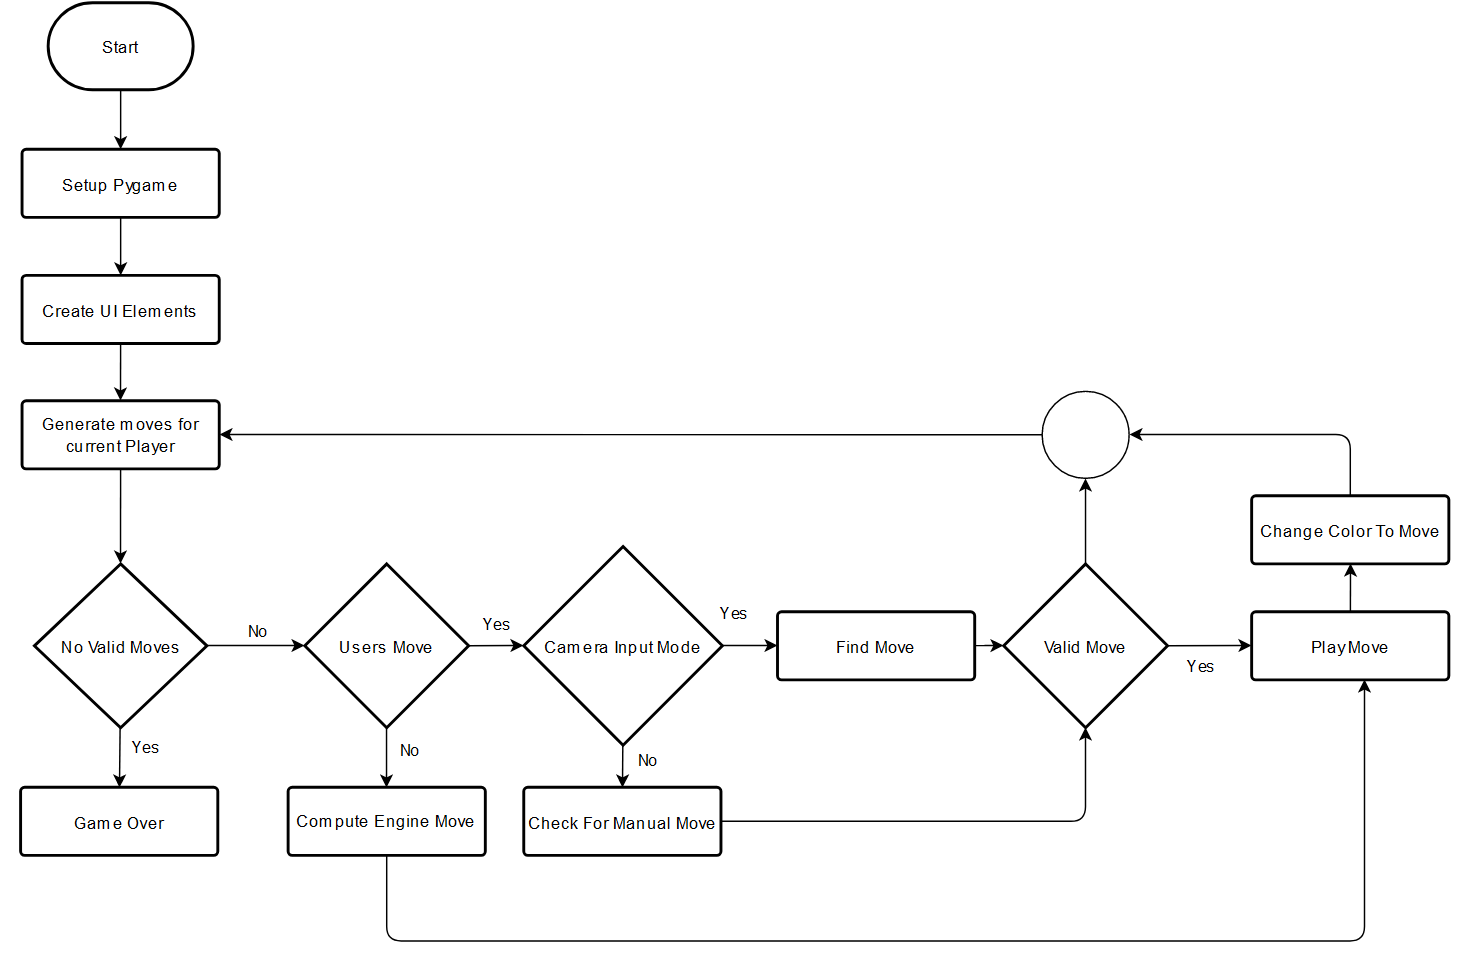
\includegraphics[scale=0.45]{images/game_loop_flowchart.png}
    \caption{PyChess Gameloop}
\end{figure}
\subsection{Voreinstellungen}
Nach Starten des Spiels wird das Spiel initialisiert. In dieser Initialisierung wird die Farbe des Spielers und des Computers bestimmt. 
Anschließend wird die Kamera des Nutzers aktiviert und der Nutzer kann die Ecken des Schachbretts markieren. Eine weitere Möglichkeit ist, das Schachbrett 
automatisch zu erkennen, jedoch wurde sich aufgrund von nachfolgenden Gründen dagegen entschieden.
\begin{figure}[H]
    \centering
    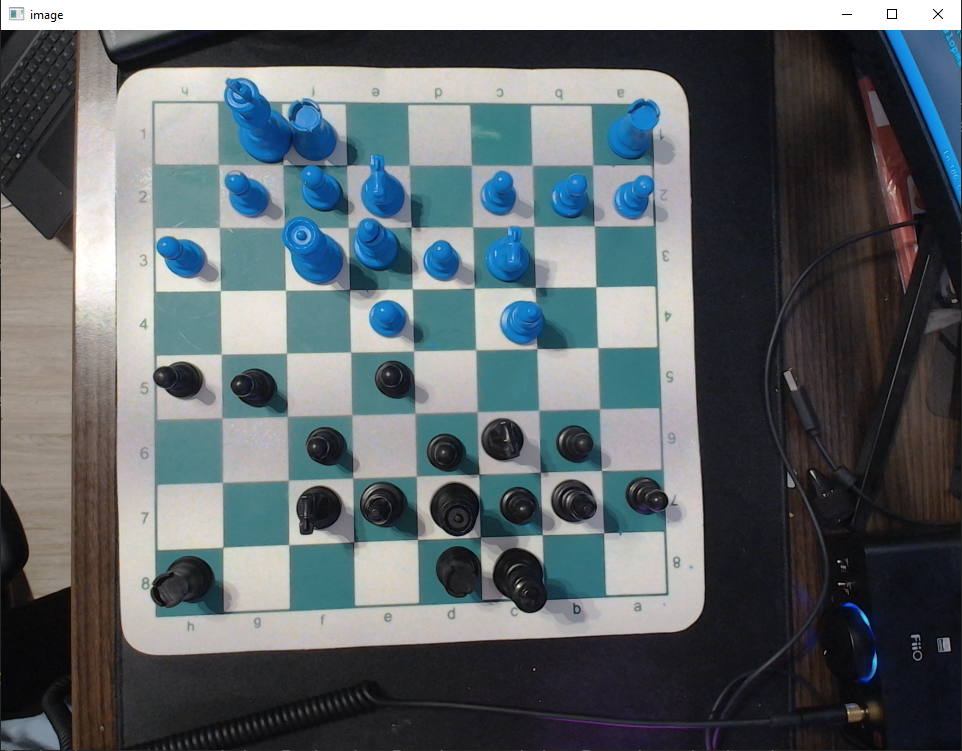
\includegraphics[scale=0.45]{images/scan_for_chessboard.png}
    \caption{Schachbrett markieren Dialog}
\end{figure}

Nachdem das Schachbrett markiert wurde, erscheint ein weiterer Dialog. In diesem wird einerseits das markierte Brett, sowie ein Dialog 
zum Einstellen der Farbregulierung angezeigt.
\begin{figure}[H]
    \centering
    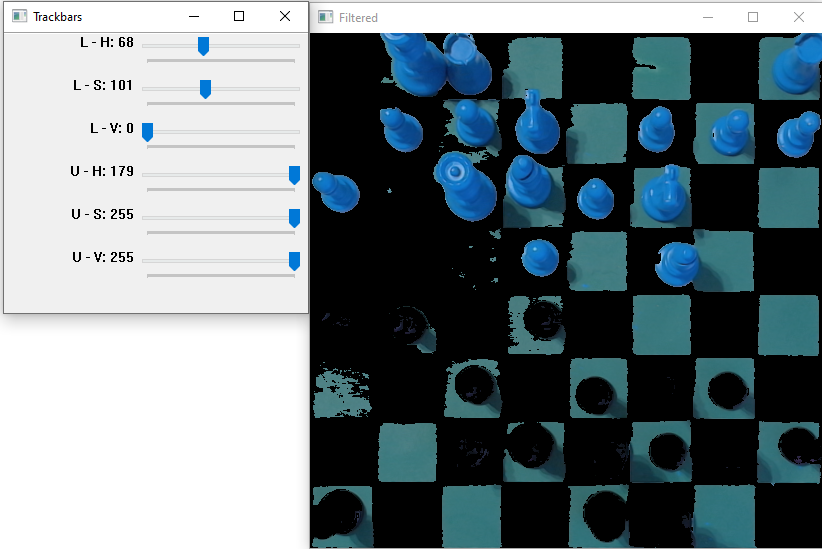
\includegraphics[scale=0.45]{images/color_filter_selection.png}
    \caption{Farbfilter Dialog}
\end{figure}

Mithilfe der Slidern, können die oberen und unteren Grenzen des HSV-Farbfilters gesetzt werden. Über das live Bild des Schachbretts wird angezeigt, wie sich die 
Einstellungen auswirken. Der Nutzer kann dann individuell auf das Schachbrett angepasst, die Werte so setzen, dass nur noch seine eigenen Spielfiguren zu sehen sind.
Dieser Schritt ist von großer Bedeutung für die spätere Zugerkennung.

Nachdem der Nutzer den Filter bestätigt hat, werden die restlichen \ac{UI} Elemente erstellt und die GUI angezeigt. 
\begin{figure}[H]
    \centering
    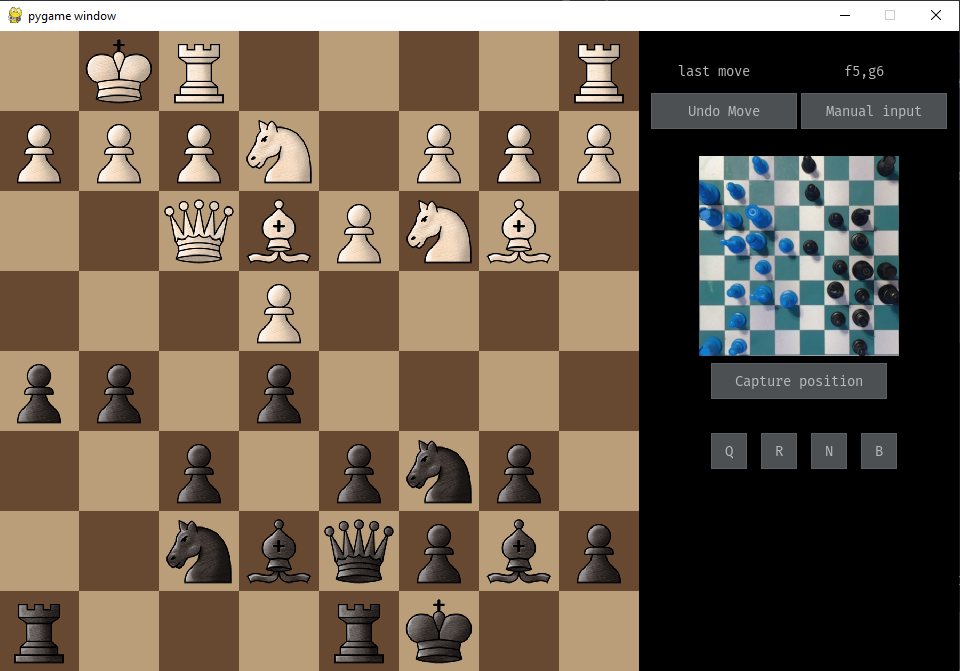
\includegraphics[scale=0.6]{images/pychess_window.png}
    \caption{PyChess Game GUI}
    \label{fig:PychessGUI}
\end{figure}

\subsection{Gameloop}
Ab hier beginnt die Gameloop. Am Anfang jeder Iteration werden alle validen Züge des aktuellen Spielers generiert und in einer Liste gespeichert.
Wenn diese Liste leer ist, also der Spieler keine Züge mehr hat, ist das Spiel zu Ende. 

\subsection{Zugerstellung}
Die Züge werden über die Funktion \(generate\_moves\) des \(moveGenerator\) Objekts erstellt.
\begin{figure}[H]
    \centering
    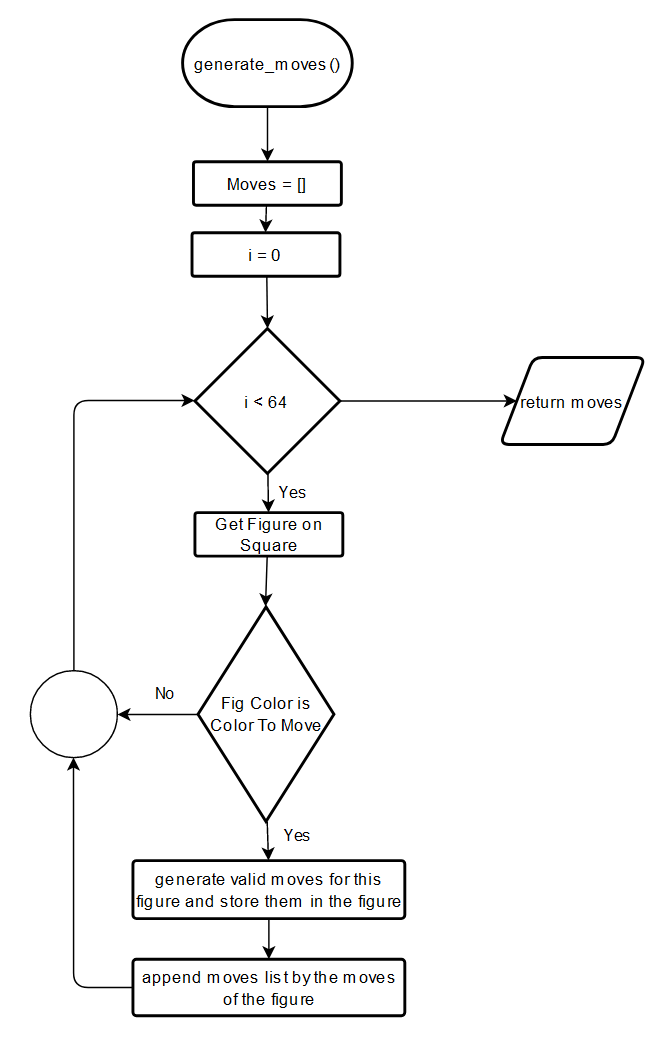
\includegraphics[scale=0.6]{images/generate_moves_function.png}
    \caption{Generierung der validen Spielzüge}
\end{figure}

Je nach Typ der Figur werden verschiedene Funktionen genutzt, um die validen Züge zu erstellen. Das Prozedere ist jedoch ähnlich.
Von einer Position ausgehend sind die Felder, auf die sich eine Figur bewegen kann immer einen bestimmten Offset entfernt.
Angenommen die aktuelle Figur ist ein König, der auf dem Feld 27 steht. Von diesem Feld ausgehend, haben die anliegenden Felder immer den gleichen Abstand in Bezug auf die Startposition.
\begin{figure}[H]
    \centering
    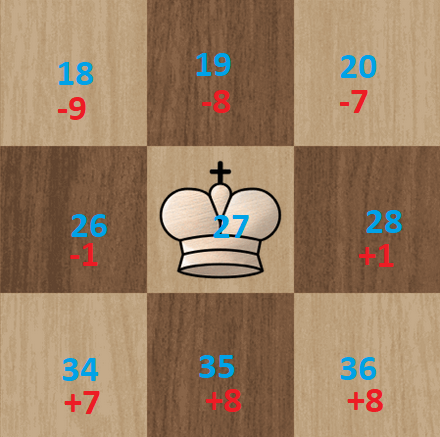
\includegraphics[scale=0.3]{images/offset_king.png}
    \caption{Figuren Offset König}
\end{figure}

Bei einem König sind damit alle vorerst validen Züge ausschließlich der Rochade abgedeckt. Bei Läufern, Türmen und Damen können die jeweiligen Offsets mit einer 
sich iterativ erhöhenden Anzahl an schritten multipliziert werden.
Springer haben einen anderen Offset als ein König, aber folgen demselben Prinzip. Nachdem diese Züge bestimmt wurden, wird ermittelt, ob der Zug legal ist.
Wenn eine eigene Figur das Feld belegt ist der Zug illegal und wird direkt verworfen und die Iteration für den Offset gegebenenfalls beendet. 
Wenn eine gegnerische Figur das Feld besetzt wird der Zug nicht direkt verworfen, aber die Iteration für das aktuelle Offset der jeweiligen Figuren beendet 
und der nächste Offset wird durchiteriert. 
Bei den Bauernzügen ist es wichtig, dass nur diagonal geschlagen werden kann und sich sonst nur ein Feld vorwärts bewegt werden kann.
Eine weitere Prüfung findet statt, ob der Zug am Ende des Brettes ist. Ohne diese Überprüfung wäre es möglich aus dem zum Beispiel linken Rand auszubrechen und rechts wieder
ins Spiel zu kommen.

\subsubsection{Spezialzüge}
Der erste Zug jedes Bauern ist hierbei eine Ausnahme, da er sich dort zwei Felder vorwärts bewegen kann. Das wird durch das Attribut \(has\_moved\) der Figur überprüft.
Der Spezialzug \(en~passant\) muss ebenfalls beachtet werden.
Dieser Tritt auf, wenn ein gegnerischer Bauer sich im letzten Zug zwei Felder nach vorne bewegt hat, und nun neben dem eigenen steht. Dann kann der gegnerische Bauer 
im Vorbeilaufen geschlagen werden. Das Feld, auf dem \(en~passant\) geschlagen werden kann wird nach jedem Zug in dem Schachbrett Objekt neu gesetzt.

\begin{figure}[H]
    \centering
    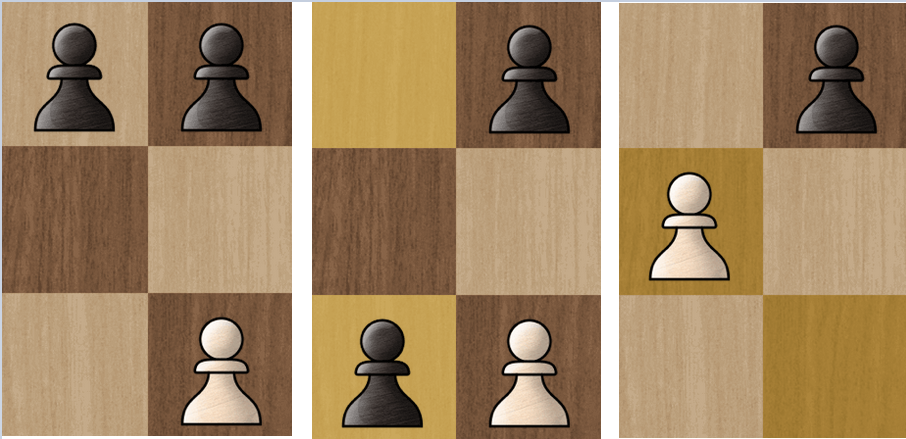
\includegraphics[scale=0.3]{images/en_passant.png}
    \caption{En Passant}
\end{figure}

Sollte ein Spieler mit dem Bauer auf die letzte Reihe kommen, kann er diesen zu einer beliebigen Figur, außer König und Bauer umwandeln.
Der letzte Spezialzug im Schach ist die Rochade, bei der ein Doppelzug von König und Turm vorliegt. Der König bewegt sich dabei zwei Felder in Richtung
des eigenen Turms und der Turm stellt sich hinter den König. Die Voraussetzungen hierfür sind, dass sich König und Turm nicht bewegt haben und der 
König nicht über ein Feld läuft, das vom Gegner kontrolliert wird. 

\begin{figure}[H]
    \centering
    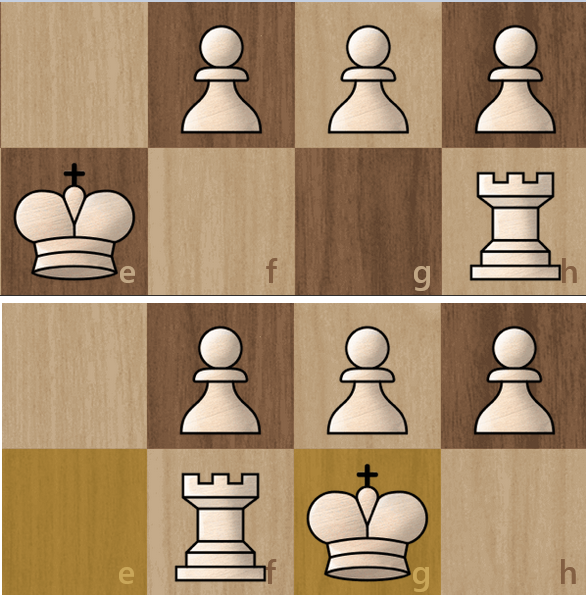
\includegraphics[scale=0.3]{images/rochade.png}
    \caption{Rochade}
\end{figure}

Jeder Zug hat ein Startfeld und ein Endfeld und eine Figur, die sich bewegt. Manche Züge haben jedoch noch weitere Flags. 

\subsubsection{Zug-Flags}
Wenn eine gegnerische Figur geschlagen wird, wird dessen Position in dem \(CAPTURE\) Attribut gespeichert. Dies dient dazu, dass auch bei \(en~passant\) die richtige 
Position der zu schlagenden Figur bekannt ist. Sollte ein Bauer sich zwei Felder vor Bewegen, so wird das neue \(en~passant\) Feld gesetzt, ansonsten wird das alte gelöscht.
Sollte der Bauer auf die letzte Reihe kommen, so wird ein flag gesetzt, welches dies widerspiegelt. 
Bei einer Rochade wird der ein Boolean gesetzt und der Typ der Rochade deklariert. Der Typ variiert hierbei zwischen einer Rochade in Richtung des Damenflügels und Königflügels.

Nach diesen Evaluierungen sind alle vorerst legalen Züge bekannt. Jedoch darf der König nach einem Zug niemals in Schach stehen, also von einer gegnerischen Figur 
angegriffen werden. Um dies zu verhindern, wird bevor der Zug gespeichert wird, er einmal ausgetestet und geprüft, ob der König anschließend angegriffen wird.
Ist das der Fall, wird der Zug aufgrund von Invalidität verworfen, ansonsten ist er legal und wir übernommen.

\subsection{Zug des Spielers}
Wenn der Spieler am Zug ist, kann er entweder über die GUI per drag and drop die gewünschte Figur bewegen, 
oder über die Kamera einen Zug am Brett spielen und diesen einlesen. Der Nutzer kann den Input durch den Button oben rechts in der UI ändern.
Je nach Modus wechselt der Name des Buttons zwischen \(Manual~input\) und \(Video~input\).

\begin{figure}[H]
    \centering
    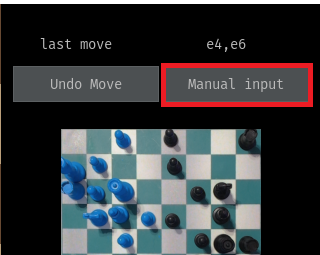
\includegraphics[scale=0.8]{images/manual_camera_input_button.png}
    \caption{Auswahl zwischen manuellem Zug und Kamera}
\end{figure} 

\subsubsection{Manueller Zug}
Die Position des Mauszeigers wird kontinuierlich erfasst. Sollte der Nutzer sich für einen manuellen Zug entscheiden, kann er eine Figur durch Klicken und halten auswählen 
und auf die neue Position ziehen. Die validen Züge werden ihm nun in Grün markiert. Der Zug kann verworfen werden, indem die Figur auf einer invaliden Stelle losgelassen wird 
und durch das Loslassen an einer validen Stelle gezogen werden.
Durch das Loslassen der Figur wird das Feld unter dem Mauszeiger ermittelt und anschließend geprüft, ob es sich hierbei um einen legalen Zug handelt.
Das geschieht, indem die Startposition und Endposition mit denen eines Zuges in der Liste der validen Züge einer Figur übereinstimmen. Wenn das der Fall ist, 
wird dieser Zug als Variable vom Typ \(Move\) zurückgegeben. Das hat den Vorteil, dass so auch die jeweiligen flags in dem Zug verankert sind.

\begin{figure}[H]
    \centering
    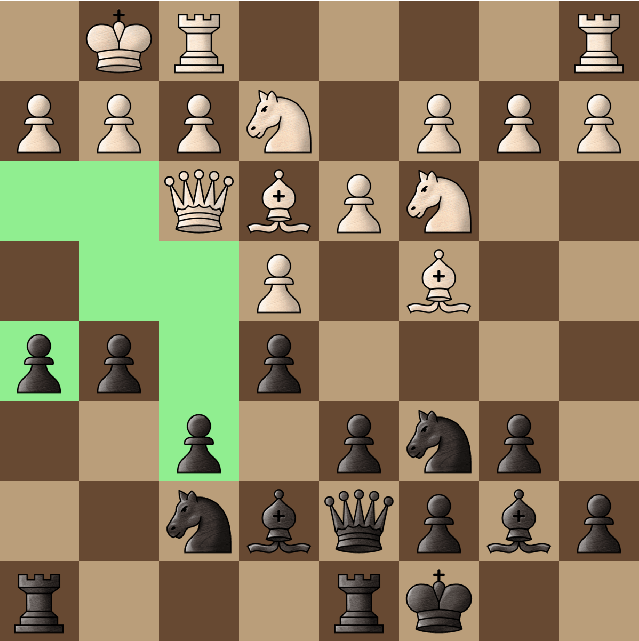
\includegraphics[scale=0.5]{images/manual_input.png}
    \caption{Auswahl zwischen manuellem Zug und Kamera}
\end{figure} 

\subsubsection{Zug durch Bildaufnahme}
Sollte ein Zug per Bildaufnahme getätigt werden, muss der Nutzer zuerst die aktuelle Position abspeichern. 
Das geschieht über das Klicken auf den Knopf \(Capture~position\). Es wäre ebenfalls möglich die aktuelle Position direkt zu speichern, ohne dass der Knopf
betätigt werden muss, jedoch kann dies zu Problemen führen. Wenn der Computergegner einen Zug macht, der eine Figur des Spielers schlägt und der Spieler dann 
den Computerzug nachspielt, anschließend sein eigenen und dann die neue Position aufnimmt, führt dies zu Problemen in der Zugerkennung.
Die Funktionalität ist deshalb so gewählt, dass der Nutzer nach dem Computerzug Zeit hat, diesen Zug zu spielen und anschließend die initiale Position aufzunehmen.

\paragraph{Bildaufnahme}
Der Knopf führt dann die Funktion \(capture\_image()\) von dem \(chessCam\) Objekt aus und speichert das Ergebnis in einer Liste \(positions\).
Die Funktion nutzt dabei die Kamera und liest das aktuelle Bild ein. Dank der vorher ausgewählten Ecken des Schachbretts kann nun eine vier Punkte Transformation 
ausgeführt werden, um nur das Schachbrett aufzunehmen und abzuspeichern.
\begin{figure}[H]
    \centering
    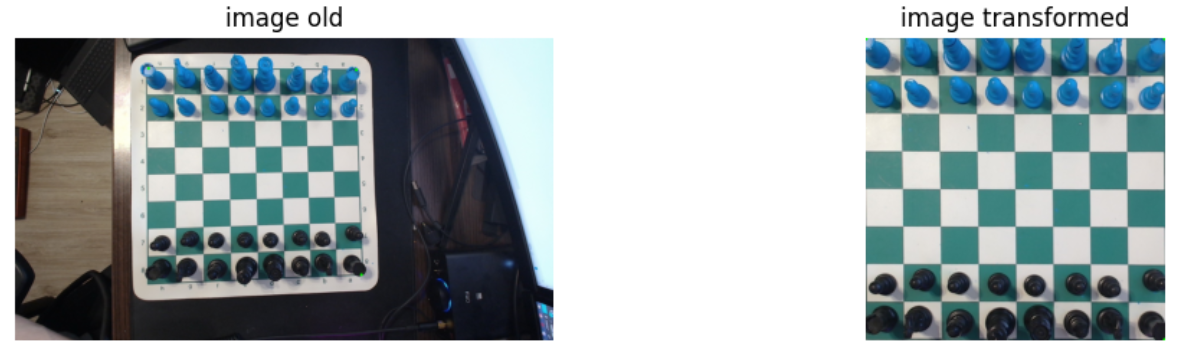
\includegraphics[scale=0.5]{images/transformed_image.png}
    \caption{Vier Punkte Transformation}
\end{figure} 

\paragraph{Zugerkennung}
Nachdem der Nutzer seinen Zug gemacht hat, kann er erneut auf den Knopf drücken und die zweite Position einlesen.
Sobald zwei Positionen eingelesen wurden, wird der Zug ermittelt. Dies geschieht über die Funktion \(get\_move(positions)\).
Diese Funktion des \(chessCam\) Objekts vergleicht die Positionen und gibt den gefundenen Zug als String zurück.

Als Erstes werden die beiden Bilder vorverarbeitet und dadurch die Figuren des Gegners und alle Felder ausmaskiert. Das geschieht über die Werte, die 
der User am Anfang gesetzt hat. Anschließend wird ein Gaußscher Unschärfefilter verwendet, um Unreinheiten zu verwaschen. 
\begin{figure}[H]
    \centering
    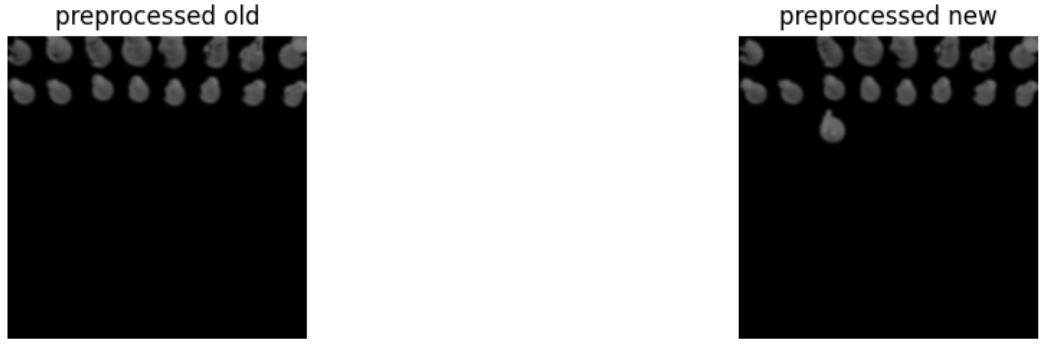
\includegraphics[scale=0.5]{images/preprocessed_image.png}
    \caption{Bildvorverarbeitung}
\end{figure} 

Nachdem die Vorverarbeitung abgeschlossen ist, wird nun die Differenz der beiden Bilder gesucht.
Das geschieht in der Funktion \(compute\_difference(image\_old, image\_new)\). In dieser Funktion wird zunächst der absolute Unterschied zwischen den Bildern 
Pixelweise berechnet. Danach wird ein Schwellenwert auf das erzeugte Bild angewendet. Jeder Pixel dessen Intensität über dem gesetzten Schwellenwert liegt,
wird auf den maximalen Wert gesetzt. Alle anderen Pixel werden auf 0 gesetzt. 
Mithilfe eines Kernels und der OpenCV \(dilate\) Funktion werden weiße Bereiche im Bild vergrößert.
Als Letztes kommt die Erosion, das Gegenstück der \(dilate\) Funktion. Diese Entfernt kleine weiße Pixel. Im Zusammenspiel mit der \(dilate\) Funktion
dient sie dazu, das Rauschen zu verringern.

\begin{figure}[H]
    \centering
    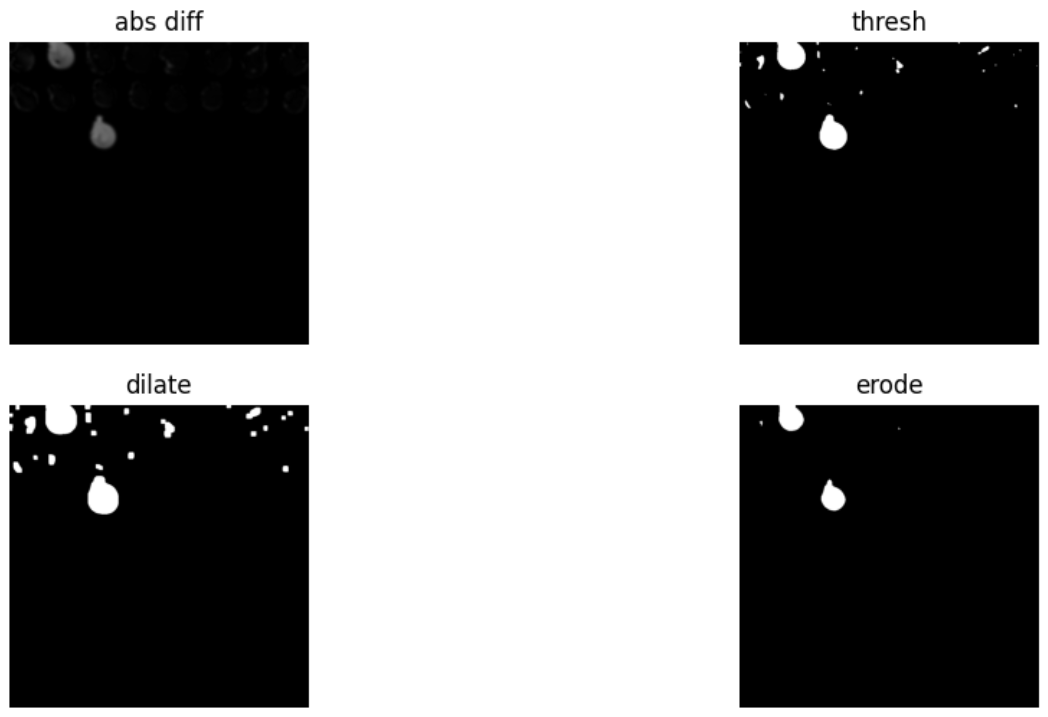
\includegraphics[scale=0.4]{images/compute_difference.png}
    \caption{Berechnung der Unterschiede in den Bildern}
\end{figure} 

Aus dem letzten Bild werden nun die Konturen durch die Funktion \(get\_contours\) extrahiert.  
Die Funktion gibt nur die Konturen und kein Bild zurück. Eine Visualisierung der Konturen würde wie die weiße Umrandung im folgenden Bild aussehen.
\begin{figure}[H]
    \centering
    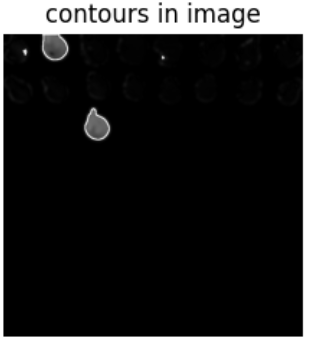
\includegraphics[scale=0.6]{images/contours_in_image.png}
    \caption{Konturen im Bild}
\end{figure} 

Mithilfe dieser Konturen und einer OpenCV Funktion, die dessen Fläche ausrechnet, werden jetzt die Bildunterschiede auf Züge gemappt. 
Dabei wird zunächst ein leeres Array, welches die Züge beinhalten soll, initialisiert. Dann werden alle Konturen durchgegangen und deren Fläche berechnet.
Sollte diese kleiner als ein bestimmter Wert sein, wird sie verworfen. 
Die Iteration über die Konturen wird so lange wiederholt, bis mindestens zwei Züge gefunden werden, oder 500 Iterationen durchgelaufen sind. 
Es ist wichtig, dass nicht auf genau zwei Züge abgefragt wird, da sonst eine Rochade zu Fehlern führen kann.
Bei jeder erneuten Iteration, durch die Konturen wird ein Zähler erhöht. Die Fläche, die eine Kontur braucht, wird mit jeder Iteration exponentiell kleiner und wird 
über eine selbst erstellte Funktion berechnet.

\begin{figure}[H]
    \centering
    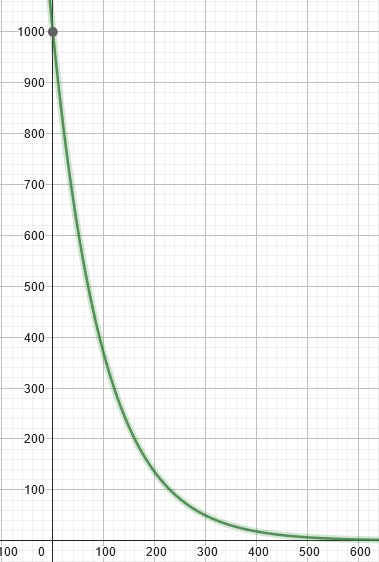
\includegraphics[scale=0.6]{images/contour_area_graph.png}
    \caption{Funktion für die Konturen-Größe $f(x) = 1000 \cdot e^{-0.01x}$}
\end{figure} 

Sollten eine Kontur gefunden werden, ein Rechteck um die Kontur erstellt und dessen Mittelpunkt berechnet. 
Da auf dem Bild nur das Brett zu sehen ist, wird der x- und y-Wert des Mittelpunktes durch die Breite und Höhe eines Feldes, also der \((Breite~oder~Hoehe~des~Bildes)~/ 8\), 
geteilt. Somit kann das genaue Feld auf dem Schachbrett ermittelt werden. 
\begin{figure}[H]
    \centering
    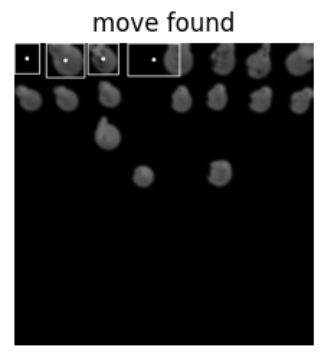
\includegraphics[scale=0.6]{images/move_found.png}
    \caption{Visualisierung des gefundenen Zuges mit Boxen}
\end{figure} 

Der ermittelte Zug wird dann als Liste der veränderten Felder zurückgegeben. Wenn die Länge der Liste zwei beträgt, handelt es sich um keine Rochade.
Nun werden alle Züge durchgegangen, bis ein Zug gefunden wurde, dessen Koordinaten mit den gefundenen übereinstimmen. Wenn das erfolgreich ist, wird der Zug gespielt, 
ansonsten wird der Typ des Inputs auf manuell gesetzt.
Wenn die Länge der Liste vier beträgt, handelt es sich um eine Rochade. Eine Rochade wird als Zug des Königs behandelt mit dem flag \(IS\_CASTLE\).
Es werden also das Start- und Endfeld des Königs herausgefunden und dann ebenfalls ermittelt, ob es sich um einen legalen Zug handelt und dieser dann gespielt.
Sollten weder zwei noch vier Züge erkannt werden, gab es einen Fehler in der Aufnahme und der Typ des Inputs wird ebenfalls auf manuell geschaltet.

Der Spieler kann jederzeit die letzten zwei Züge rückgängig machen, falls ein falscher Zug gespielt wurde. Dabei wird der vorherige Zustand des Schachbretts geladen und
alle Änderungen rückgängig gemacht. Das geht über den Knopf \(Undo~Move\) in der GUI.
\begin{figure}[H]
    \centering
    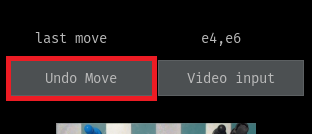
\includegraphics[scale=0.6]{images/undo_move.png}
    \caption{Zug rückgängig machen}
\end{figure} 

\subsection{Zug der Engine}
Wenn die Engine am Zug ist, wird der Zug durch die Funktion \(get\_move()\) ermittelt. Die Engine verwendet dabei die Stockfish Bibliothek und hat eine Wertung von 2000.
Durch die Klasse des Schachbretts wird ein \ac{FEN} String generiert. 

Der \ac{FEN} String ist eine Kurznotation, die jede beliebige Brettstellung widerspiegeln kann.
\(rnbqkbnr/pppppppp/8/8/8/8/PPPPPPPP/RNBQKBNR~w~KQkq~-~0~1\) beschreibt die Startstellung einer Partie. Kleingeschriebene Buchstaben stehen für schwarze die Figuren
und groß geschriebene für die weißen Figuren. Zahlen deuten die Anzahl der leeren Felder an. Schrägstriche leiten eine neue Reihe ein.
Nach den 64 Feldern steht ein Buchstabe für den aktuellen Spieler. Dabei steht \(w\) für weiß und \(b\) für schwarz. \(KQkq\) beschreibt die Rochadenrechte.
Das \(K~und~k\) steht für die Rochade auf dem Königsflügel und das \(Q~und~q\) für die Rochade auf dem Damenflügel, wobei die Groß- und Kleinschreibung wieder die Farbe
repräsentiert. Wenn kein Spieler mehr Rochieren darf, steht stattdessen ein \(-\) anstelle von \(KQkq\). Die vierte Gruppe beschreibt das \(en~passant~Feld\). 
Ein \(-\) zeigt, dass kein \(en~passant\) möglich ist und ein \(a3\) würde ein \(en~passant\) auf dem Feld \(a3\) zulassen.
Die fünfte Gruppe beschreibt die Anzahl der Halbzüge seit dem letzten Bauernzug oder schlagen einer Figur und die sechste Gruppe gibt die nächste Zugnummer an.

Der \ac{FEN} String wird generiert, indem durch das Feld iteriert wird und der Typ der jeweiligen Figur gespeichert wird und 
anschließend die anderen Informationen aus der Schachbrettklasse angehängt werden. Dieser \ac{FEN} String wird dann an die Engine gegeben und diese versucht innerhalb
einer Sekunde den besten Zug zu finden. Dieser Zug wird dann in den validen Zügen gesucht, um ihn als variable vom Typ \(Move\) zurückzugeben und 
anschließend zu spielen.

\subsection{Spielen eines Zuges}
Das Spielen eines Zuges findet in der Funktion \(make\_move(move)\) der Schachbrettklasse statt. Zunächst wird der aktuelle Spielstand gespeichert, damit er
wiederhergestellt werden kann. Im Anschluss wird der Spielzug erhöht, die Farbe des aktuellen Spielers gewechselt, das \(en~passant~Feld\) upgedatet und die Halbzüge
aktualisiert.
Sollte es sich bei dem Zug um eine Rochade handeln, wird eine andere Funktion aufgerufen, die je nach Typ der Rochade die entsprechenden Felder aktualisiert.
Ansonsten wird die gezogene Figur auf dem Spielfeld bewegt und eventuell geschlagene Figuren werden aus dem Array gelöscht.

\begin{figure}[H]
    \centering
    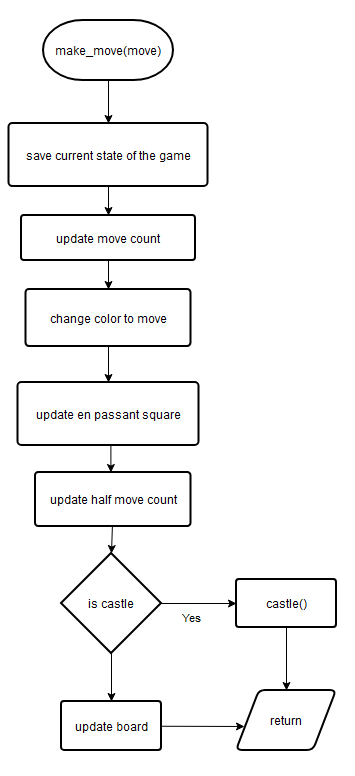
\includegraphics[scale=0.6]{images/make_move_function.png}
    \caption{Funktion zum Spielen eines Zuges}
\end{figure} 

\section{Herausforderungen im Entwicklungsprozess}
Im Verlauf der Entwicklung der Applikation traten ins besondere Probleme bei der Erstellung einer eigenen Schach-Engine und der Kameraauswertung auf.

\subsection{Engine-Entwicklung und Leistung}

\subsubsection{Zeitaufwendige Zugberechnung}
Anfangs wurde versucht eine eigene Engine zu entwickeln. Mit einer einfachen Minimax-Funktion wurden die Suchzeiten jedoch schon bei einer geringen Tiefe 
zu lang. Es wurden diverse Versuche unternommen, die Geschwindigkeit zu verbessern.

\subsubsection{Alpha-Beta-Pruning und andere Lösungen}
Ein weit verbreiteter Ansatz zur Beschleunigung der Minimax-Funktion ist das Alpha-Beta-Pruning. Dies alleine senkte die Rechenzeit der Engine drastisch, jedoch nicht genug,
um sie Nutzen zu können. Andere Optimierungsansätze, wie die Zugsortierung und das Nutzen von Transpositionstabellen hat ebenfalls zu einer nicht ausreichenden 
Leistungssteigerung geführt. Der Hauptgrund dafür ist die Zeit, die der Computer benötigt, um alle legalen Züge einer neuen Position zu berechnen.

\subsubsection{Potenzielle Alternativen}
Lösungsansätze für dieses Problem sind einerseits das Wechseln auf eine effizientere Programmiersprache, oder der Versuch die Funktion an sich effizienter zu machen. 
Beispielsweise ist es statt der Nutzung von Figuren-Objekten in einer Liste, möglich eine Integer-Liste zu nutzen, 
die Anhand ihres Wertes die Farbe, und den Typ der Figur widerspiegeln. Ein weiterer Ansatz ist es, nur die Züge der Figuren zu berechnen, die von dem letzten Zug betroffen 
sind und die anderen Züge beizubehalten. Das Potenzial für die Leistungssteigerung der Funktion ist enorm, jedoch ist die Umsetzung sehr komplex, da zu den eigentlichen Zügen
immer alle betroffenen Figuren ebenfalls berechnet werden müssen. Dies kann die gewonnene Leistungssteigerung stark absenken.

\subsubsection{Verwendung von Stockfish}
In diesem Projekt wurde sich dazu entschieden auf eine externe Engine, Stockfish, zurückzugreifen. Sie ist über eine Python Bibliothek einfach einzubinden und
neben der Leistungssteigerung gehört sie zu den stärksten Engines der Welt.

\subsection{Kamera-Blockaden und irreführende Wahrnehmungen}
Die Nutzung einer Kamera brachte ebenfalls einige Probleme mit sich. Um die Figuren zu erkennen, müssen sich diese deutlich von dem Hintergrund abheben.
Ein erster Ansatz war es, die alte Kamera durch eine Leistungsstärkere auszutauschen, was zu ersten fortschritten geführt hat. Außerdem wurde sich für 
ein Brett entschieden, dessen Farben von den der Figuren abweichen. Dadurch ist es leichter die Figuren auszumaskieren und die Züge mit einer höheren 
Präzision zu finden. Der Winkel der Kamera spielte ebenfalls eine große Rolle. Wenn dieser zu flach war, waren kleinere Figuren hinter größeren versteckt.
Um dieses Problem zu beheben wurde ein Kameraarm montiert, der es erlaubt einen Topdown-View zu erzeugen und die Züge zuverlässig zu finden.



